% !TeX program = xelatex
% !TeX encoding = UTF-8
\documentclass[UTF8]{standalone}
\usepackage{amsmath,fourier,ctex,tikz}
\begin{document}
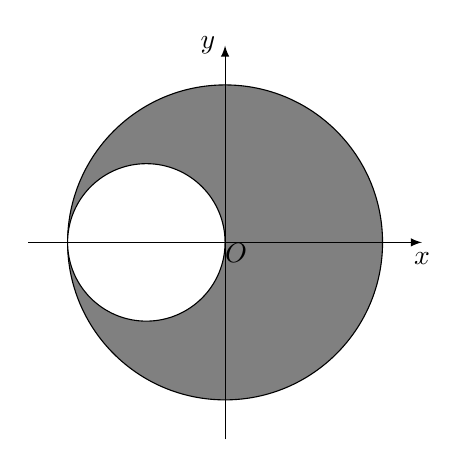
\begin{tikzpicture}
	\filldraw[fill = gray,draw = black] (0,0) circle (2);
	\filldraw[fill = white,draw = black] (-1,0) circle (1);
	\draw[-latex] (-2.5,0) -- (2.5,0) node[below] {$x$};
	\draw[-latex] (0,-2.5) -- (0,2.5) node[left] {$y$};
	\node[right=4pt,below=-3pt] at (0,0) {$O$};
\end{tikzpicture}
\end{document}